% Chapter Template

\chapter{Implementation} % Main chapter title

\label{implementation} % Change X to a consecutive number; for referencing this chapter elsewhere, use \ref{ChapterX}

\lhead{Chapter 5. \emph{Implementation}} % Change X to a consecutive number; this is for the header on each page - perhaps a shortened title

%----------------------------------------------------------------------------------------
%	SECTION 1
%----------------------------------------------------------------------------------------

%\colorbox{green}{Some introduction that motivates the work done in this thesis}

%\colorbox{green}{henvis til NS, nevn eksplisitt de ligningene som brukes}

%\colorbox{green}{Ta med et turbulensbilde, og bilde av plumen.}

This chapter aims to present the implementation done in this thesis. The main motivation 
behind the work was to see how Nek5000 works for complex geometries and to develope 
necessary tools in order to improve its functionality. 

The main tools in addition to Nek5000 needed to perform the simulations presented in this 
chapter are \textit{ANSYS ICEM} and \textit{python}. For post-prosessing \textit{Visit} and
\textit{Matlab} was used.

As shown in figure~\ref{fig:mesh} the coarse element grid is created
in ICEM and then converted using the python script \verb|mshconvert| while the
distribution of GLL-nodes and the simulation itself was 
performed in Nek5000. This procedure to generate a mesh had some limitations
for complex geometries and one part of this thesis has been to develop solutions that makes it 
possible to work with complex geometries in Nek5000.

The other part of the thesis has been to understand and apply Nek5000 with and without 
LES to turbulent flow with gas dispersion and compare the results with reference 
solutions from experiments and other solvers.

The implementation is presented in 4 chapters. The first two chapters describe two flow situations 
used to compare Nek5000 with equivalent solvers and the two last chapters describe two distinct
contributions to the mesh creating routine. 

\section{Case 1: Gas dispersion in a simplified urban area}
%The problem investigated in this work is gas dispersion of neutral gas in a velocity field through four cubic blocks.
%Similar simulations have been done in CDP and Fluent which are compared to data from a wind-tunnel experiment performed by ALAN.
The scenario investigated in this work is dispersion of a neutral gas in a rectangular tunnel
with four cubic blocks placed as obstacles. The blocks have sides $h = 0.109$m and represent a 
set of buildings forming a street canyon. The gas is released from a circular source on 
ground level and
is translated by the wind field through the canyon, see figure~\ref{fig:layout}.
In this figure $h$ have been used as the length scale. The dotted lines
indicates the positions where data is collected.
%
\begin{figure}[h]
	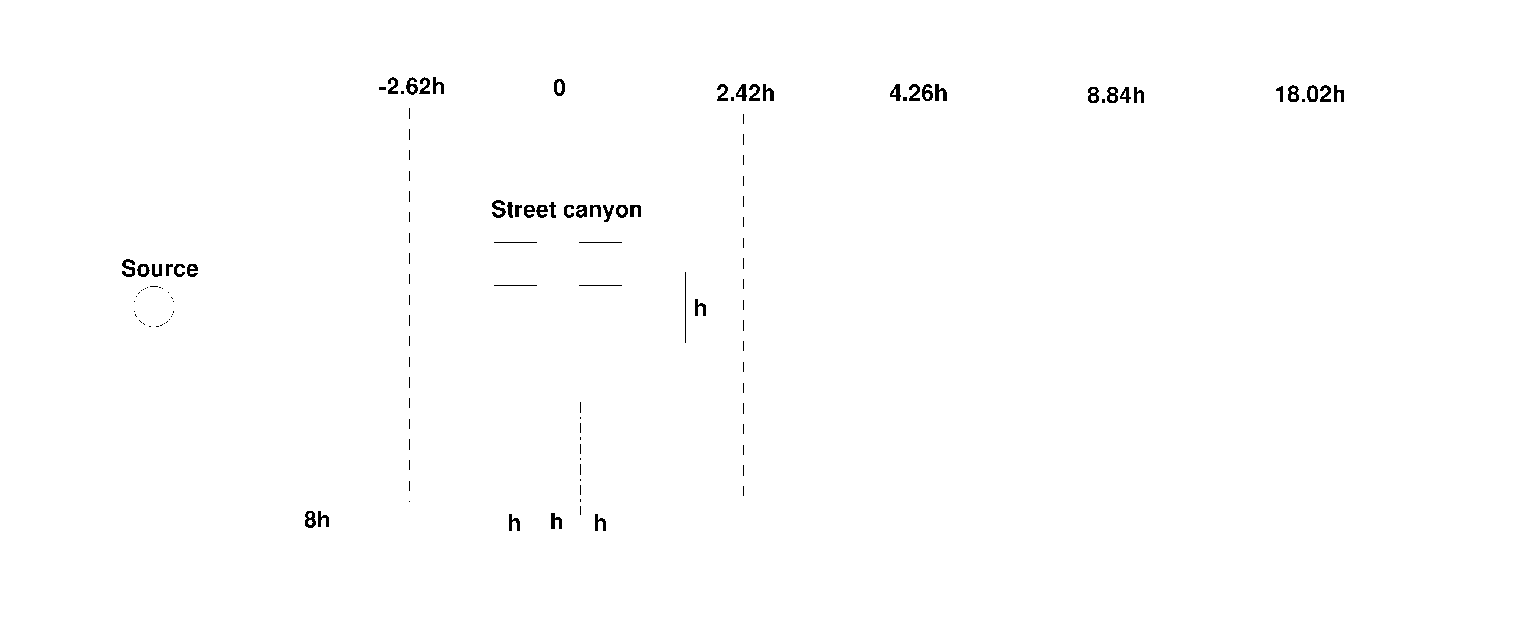
\includegraphics[width=1.1\textwidth]{Figures/layout.eps}
	\caption{Schematic overview of the domain from above. The data is collected along the dotted lines.}
	\label{fig:layout}
\end{figure}
%

Scaling the domain with the size of the boundary layer $H =1$m restricts it to
the box $0.0\leq x/H \leq 4.96,-1.75\leq y/H \leq 1.75, 0\leq z/H \leq 1.5$.
The four cubic boxes are centered around $(1.4315,0)$ with a distance $h$ between each box.
The source is placed with its center in $(0.396,0)$ and radius $r = 0.0515$.
The grid used for the computations consists of 14747 elements and with a polynomial degree of
8 the total number of nodes $N\approx 7,6$mill. 


The simulations are performed using Large Eddy Simulation (LES) 
with the dynamic Smagorinsky-Lilly subgrid-scale model and by applying the polynomial filtering
routine which is available in Nek5000. 
The release of gas will result in a plume that is advected with the wind field,
see figure~\ref{fig:plume}. The concentration of the released gas at the 
indicated positions in figure~\ref{fig:layout} are compared with 
experimental data and simulations performed in CDP\@. 
The wind-field in the tunnel is created by an inflow condition that is defined from previous 
simulations in CDP~\cite{eriksson}.
For clarification some of the variables repeatedly mentioned throughout this thesis will be 
stated explicitly in table~\ref{tab:simplevariables}.
\begin{table}
    \centering
    \begin{tabular}{c c c c}
        Variable & value & unit & commentary \\ \hline
        $H$   & $1$ & m & length scale of the domain \\ 
        $h$   & $0.109$ & m & the sides of the cubic boxes\\ 
        $Q$   & $50$ & dm$^3$/min & gas release from source \\ 
        $U_{ref} $*& $\approx1.08$ & m/s & reference value of $U$ \\
    \end{tabular}
    \caption{Essential variables, *this value is calculated as a time average of the velocity in 
        x-direction at a point far away from the floor and walls and will therefore 
        vary a small amount from case to case. }
    \label{tab:simplevariables}
\end{table}

The inflow conditions had to be extrapolated onto the domain at each time step. To mimic the situation in the wind-tunnel the velocity field
on the inflow was generated in a different simulation performed in CDP. The inflow velocity was written to file every 
$0.0013$s for a total of $28$s and had to be interpolated onto the domain for the simulations in Nek5000 since the grid was not identical.
The right plot in figure~\ref{fig:inflow} is an instantanous picture of the inflow velocity in x-direction, 
notice how the pattern repeats itself along the y-axis. This is because the inflow data was generated in a smaller channel, $\approx 1/3$ of the 
width of the computational domain used for the data sampling. An interpolation algorithm had to be implemented in order to adjust 
the inflow-data to the computational mesh, this was done directly in \verb|.usr|. 
%
\begin{figure}
\centering
  \centerline{
\begin{minipage}{.6\textwidth}
  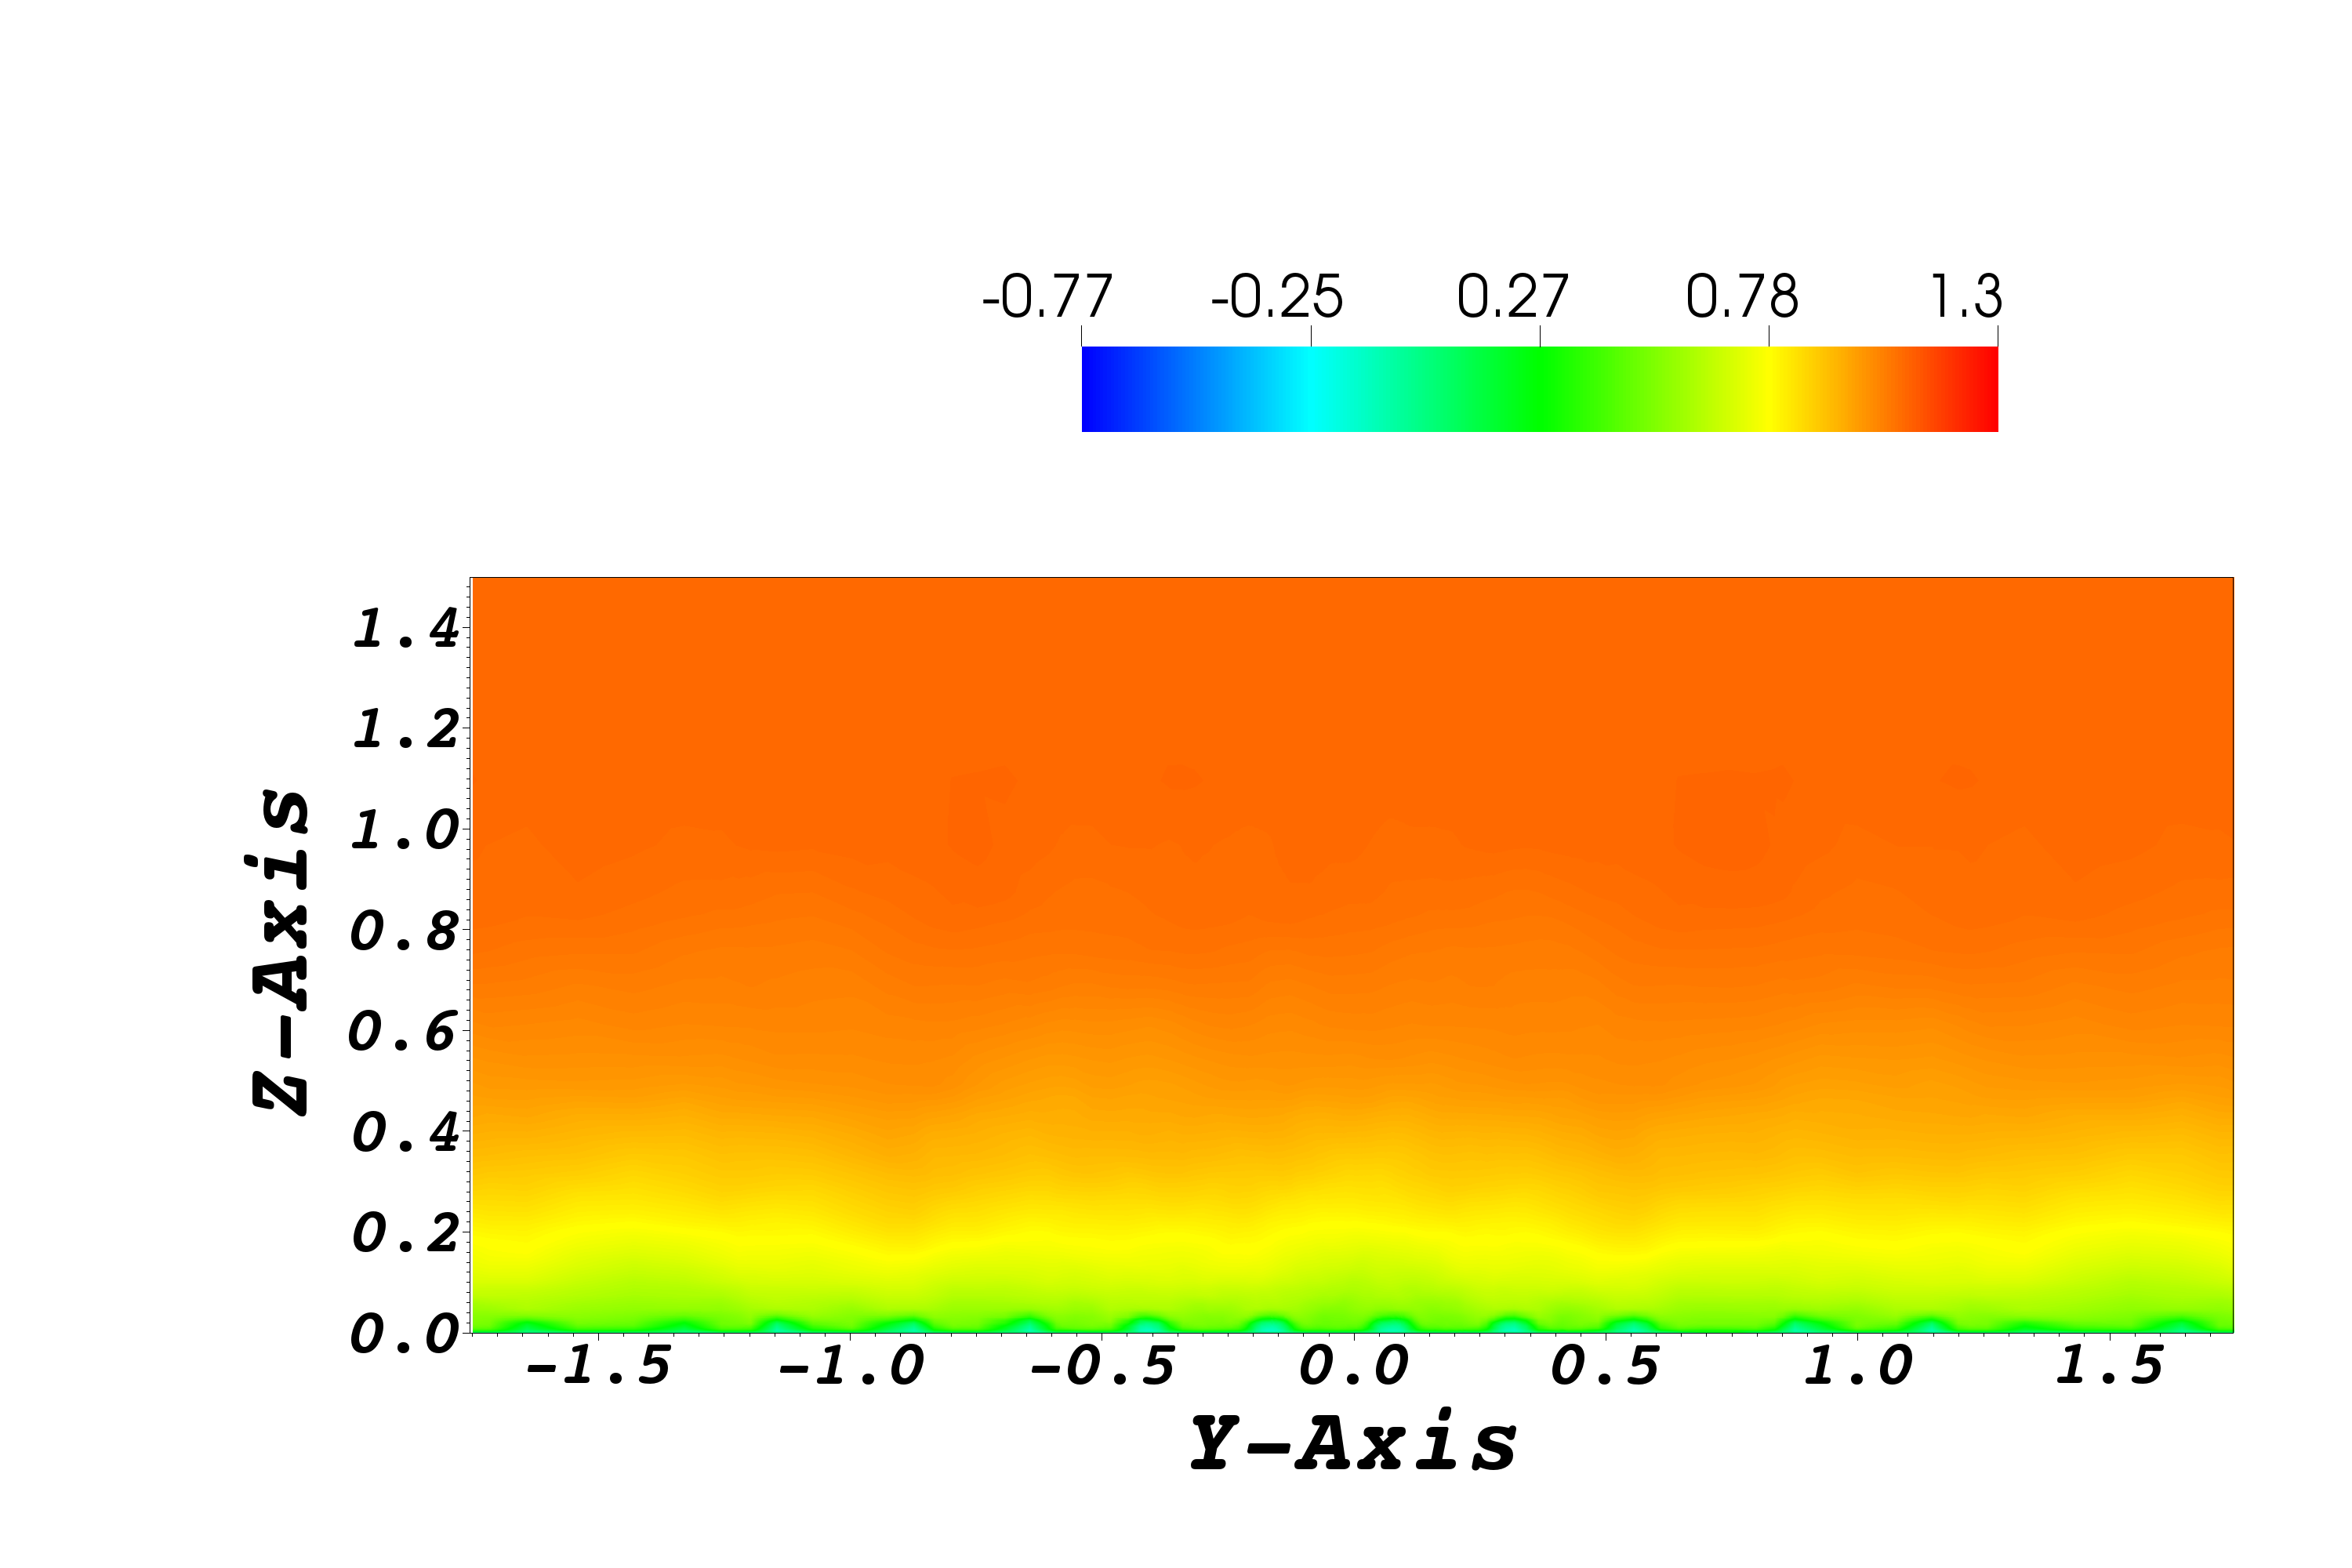
\includegraphics[width=1.0\linewidth]{Figures/inflow_field_avg.png}
  %\captionof{figure}{A figure}
\end{minipage}%
\begin{minipage}{.6\textwidth}
  \centering
  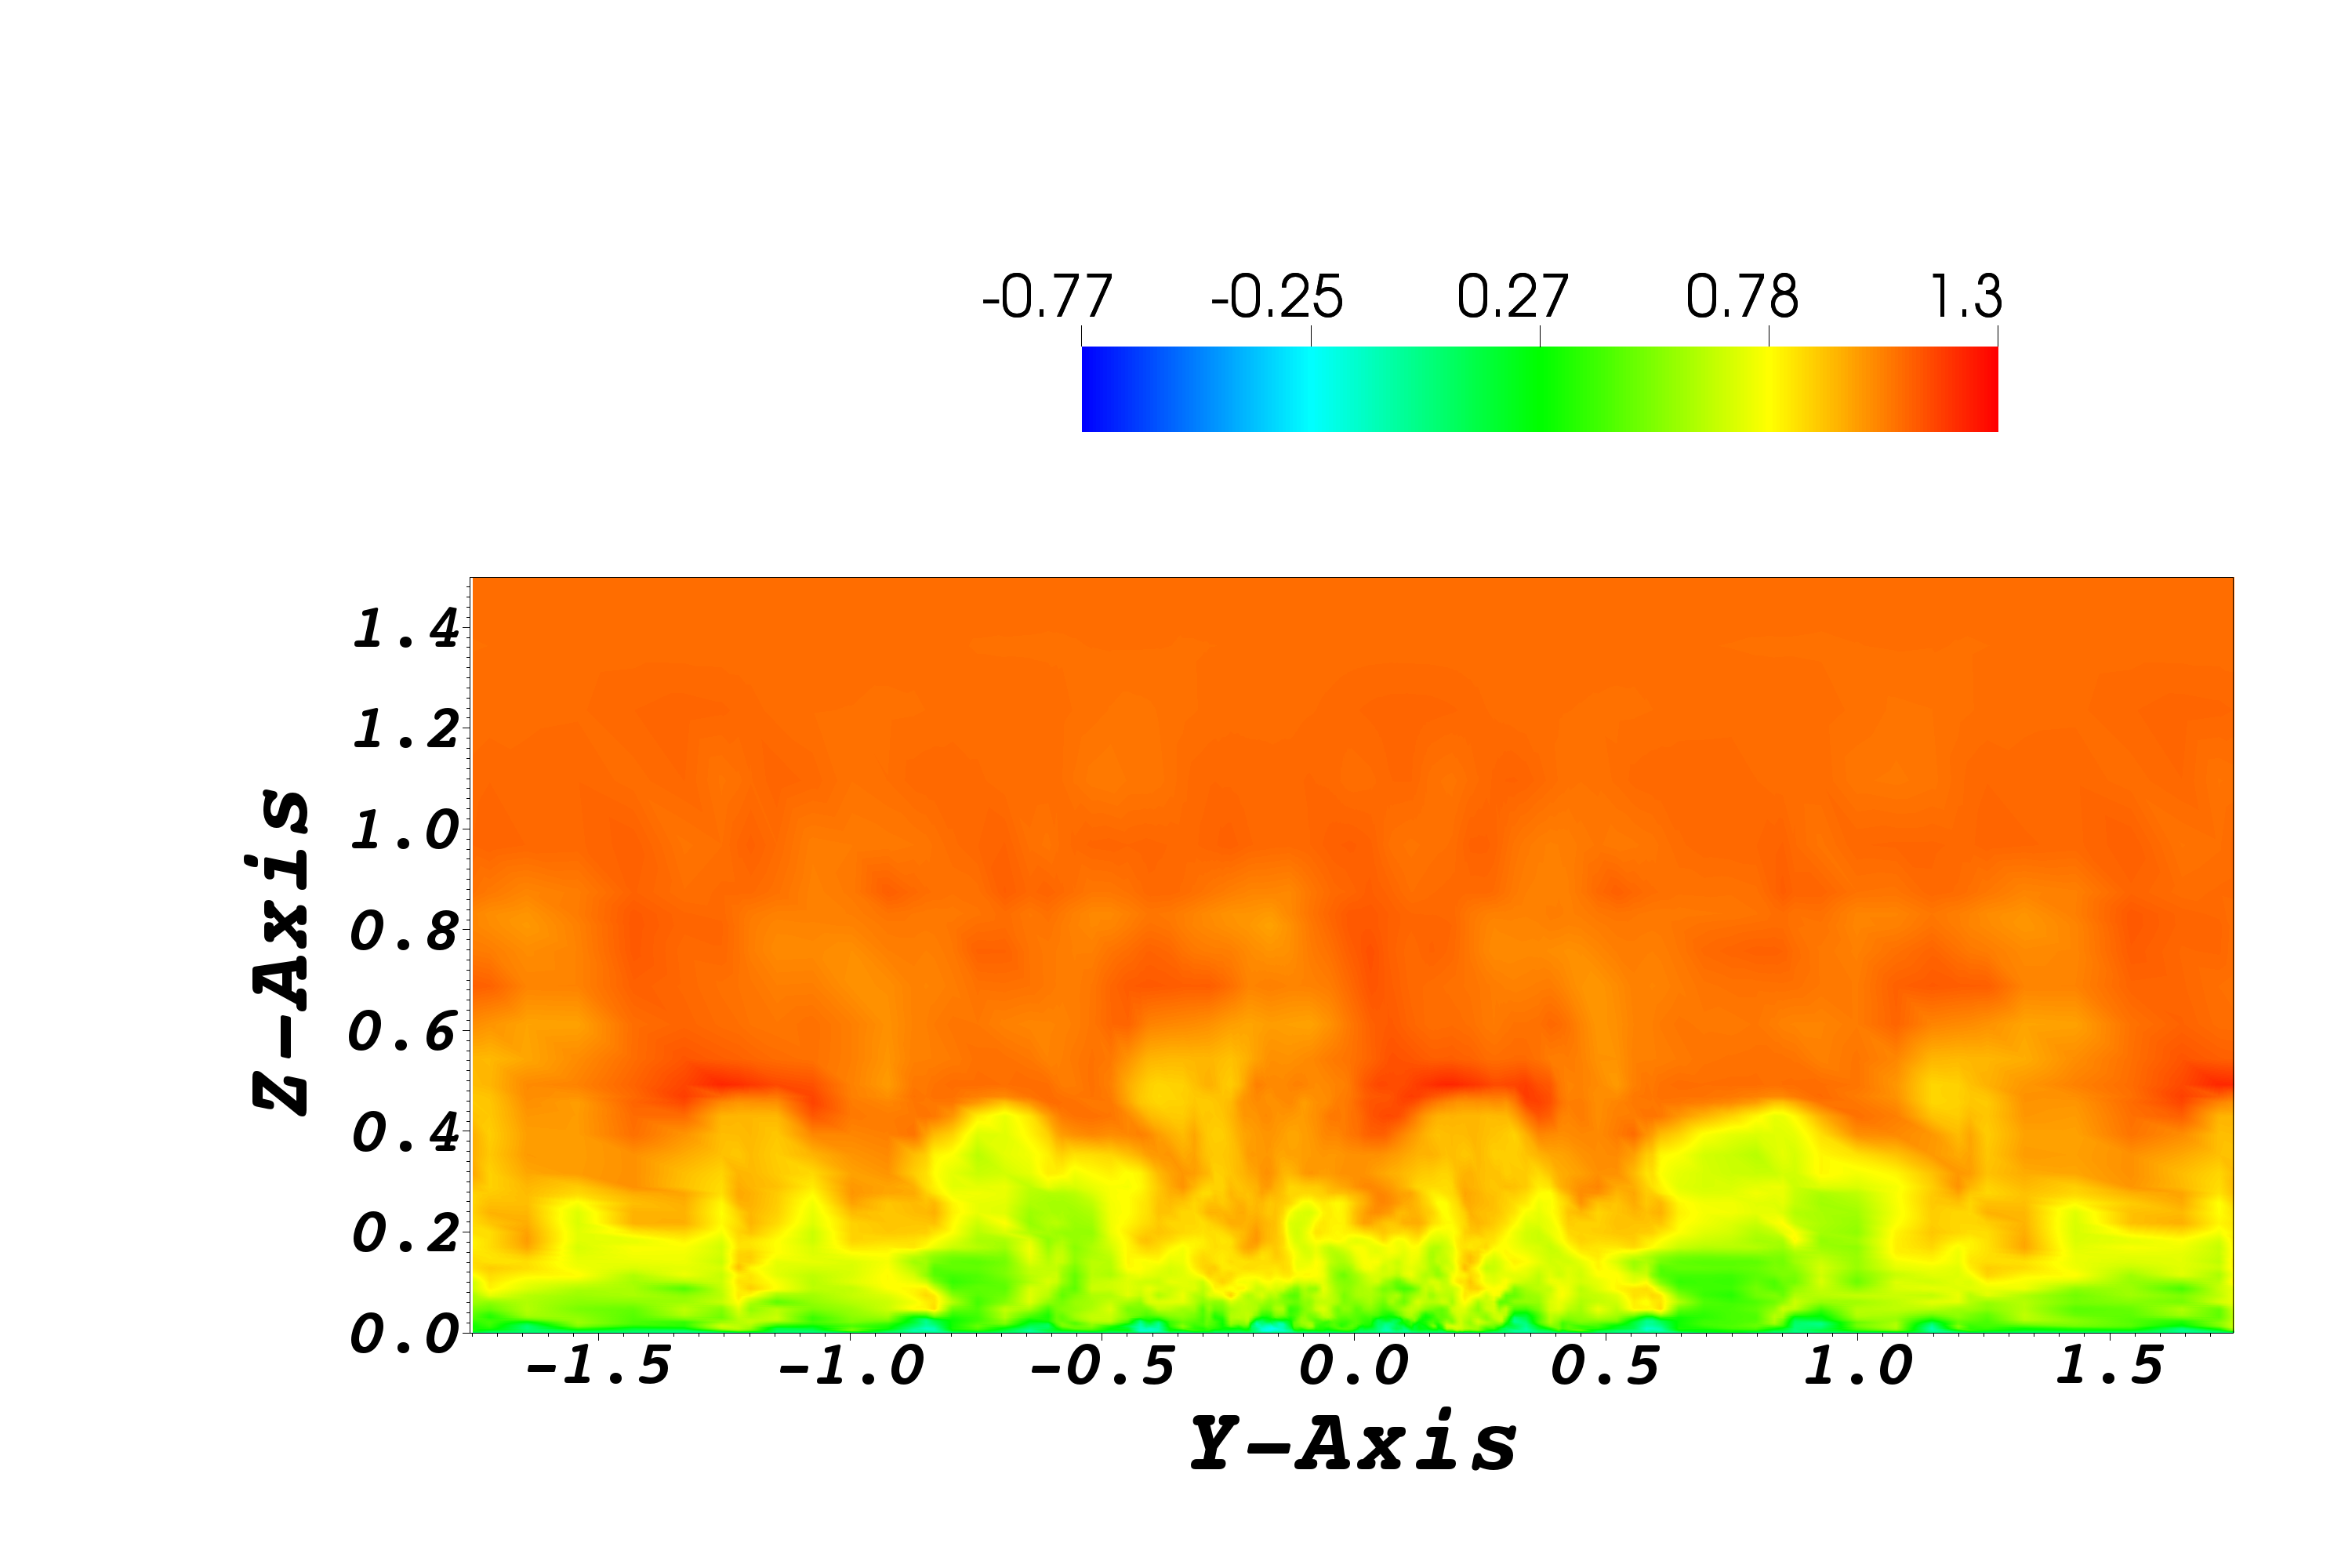
\includegraphics[width=1.0\linewidth]{Figures/inflow_field.png}
\end{minipage}
}
  \caption{The averaged (left) and instantaneous (right) x-velocity on the inflow boundary.}
  \label{fig:inflow}
\end{figure}
%

The simulation in Nek5000 was performed in the following manner; first 6 seconds of initialization of the velocity field in the 
channel, followed by 8 seconds of gas release to initialize the gas-concentration. After assuring that the wind-field was 
correctly created and the released gas had reached the measurement lines furthest from the source the data sampling of 22 seconds 
started.
%
\begin{figure}[h]
	\centering
	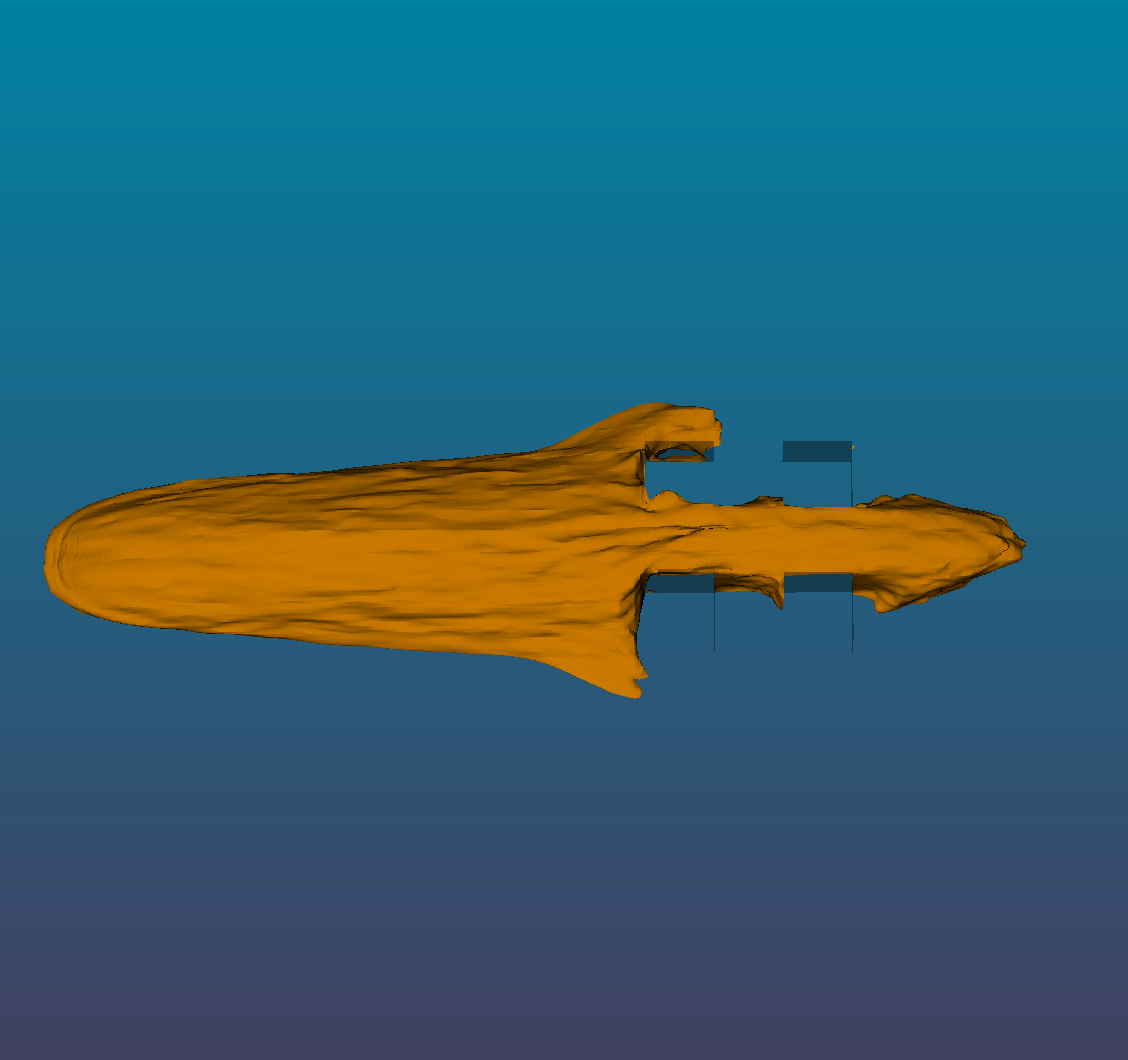
\includegraphics[width=0.6\textwidth]{Figures/plume2.png}
	\caption{An iso-surface of the average concentration with $C=0.03$ 
    after 30 seconds of sampling.}
	\label{fig:plume}
\end{figure}
%

\section{Case 2: Drag and lift on a cylinder}
A standard benchmark case for flow solvers is presented in ~\cite{benchmark}. 
The case is to calculate the drag and lift coefficients on a cylinder in a rectangular channel.
The setup for the domain and boundary conditions are given in figure~\ref{fig:cylinder}.
The constants applied in the description of the geometry and the coefficient scales are listed 
in table ~\ref{tab:case2consts}.
%
\begin{table}[h]
    \centering
    \begin{tabular}{c l l}
     Constant & Value & Property \\ \hline
    $H$ & $0.41\text{m}$ & Width and height for the channel \\
    $D$ & $0.1\text{m}$ & Diameter of the cylinder and length scale \\
    $U$ & $0.2\text{m/s}$ & Velocity scale \\
    $\nu$ &  $ 10^{-3}\text{m$^2$/s}$ & Kinematic viscosity of the fluid \\
    $Re$ & $20$ & Reynolds number \\ 
    \end{tabular}
    \caption{Constants for case 2}
    \label{tab:case2consts}
\end{table}
%
Finding the drag and lift coefficient requires a calculation of the velocity field around the cylinder
which is done by solving the unsteady N-S equations until a steady flow is reached. This implies that the
spatial accuracy will dominate the error and one would expect great results in Nek5000 
due to its spectral convergence rate.

The flow is laminar with Reynolds number $Re=20$ so all the 
challenges arising when dealing with turbulent flow does not come to play in this case. 
%
\begin{figure}[h]
    \centering
    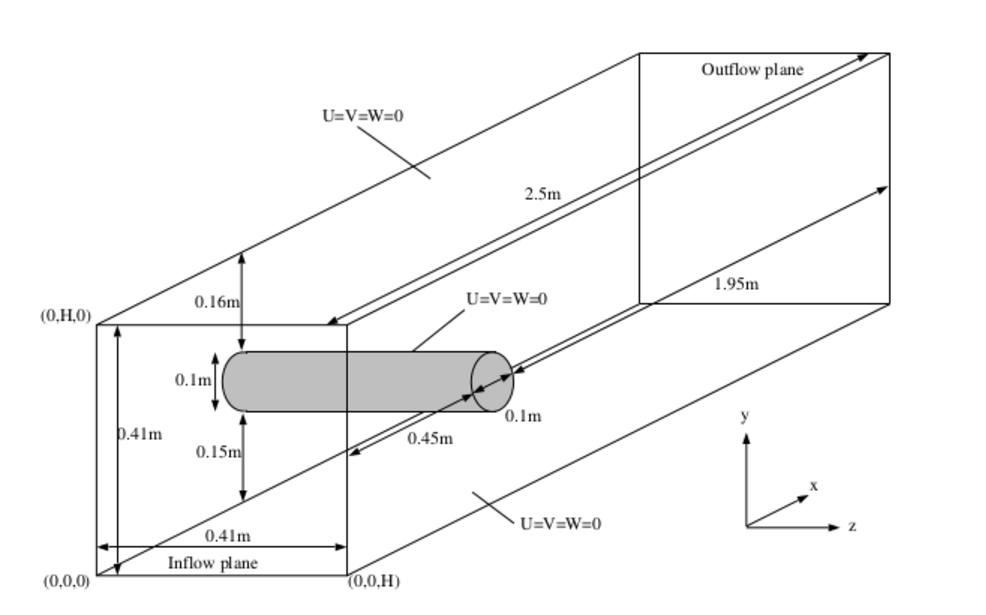
\includegraphics[width = 1.0\textwidth]{Figures/cylinder.pdf}
    \caption{Computational domain and boundary conditions.}
    \label{fig:cylinder}
\end{figure}
%
The drag and lift forces on a surface $S$ are given as 
%
\begin{align}
    F_D = \int_{S}(\rho \nu \frac{\partial v_t}{\partial n}n_y-pn_x)dS 
    \qquad , \qquad
    F_L = -\int_{S}(\rho \nu \frac{\partial v_t}{\partial n}n_x+pn_y)dS.
    \label{eq:dragnlift}
\end{align}
%
$v_t$ is the tangential velocity, $\mathbf{n}=[n_x,n_y,0]$ and the tangent velocity vector is 
defined as $\mathbf{t} = [n_y,-n_x,0]$.
is the unit vector normal to the surface $S$ 
Surface integrals in Nek5000 are solved numerically, $\int_S f dS = \sum f_i A_i$. Where $f$ is some function and $A_i$ is the areal corresponding
to the nodal value $f_i$. 

\colorbox{green}{Nevne hvordan integralet løses i Nek?? Heller skrive i appendiks??}

The coefficients corresponding to these forces known as the drag and lift coefficients 
are given by the formulas 
\begin{align}
    c_D = \frac{2F_D}{\rho U^2 D H}
    \qquad , \qquad
    c_L = \frac{2F_L}{\rho U^2 D H}.
    \label{eq:dragnliftcoeffs}
\end{align}


Nek provides functions for calculating lift and drag on any user-specified object.
The function is called \verb|drag_calc(scale)|, with the input parameter 
defined by the user, for this case \verb|scale| $=2/(\rho U^2DH)$.  
Apart from this the function \verb|set_obj()| has to be modified in order to create an object 
which consists of pointers to all the faces on the cylinder.
%Let $x,y$ be points in the computational domain, $x_c,y_c$ be the coordinates to the 
%center line in the cylinder and $0<tol\ll1$ be some user defined tolerance. The faces that belong to the cylinder can then be found by 
%looping over all elements and their faces evaluating $\epsilon = \sqrt{(x-x_c)^2+(y-y_c)}$.
%If $\epsilon < tol$ for an entire face then this face is known to 
%belong to the cylinder and is added to the object. Nek also allows the user to specify multiple objects 
%assigning the faces of interest to object 1, object 2 etc. The geometry and mesh 
%for this case was generated in ICEM, and the total number of elements are 2070. 
%For the final calculation polynomial degree $P = 11$ was applied leading to a 
%total of $N = 2755170$.
%
\begin{figure}[h]
    \centering
    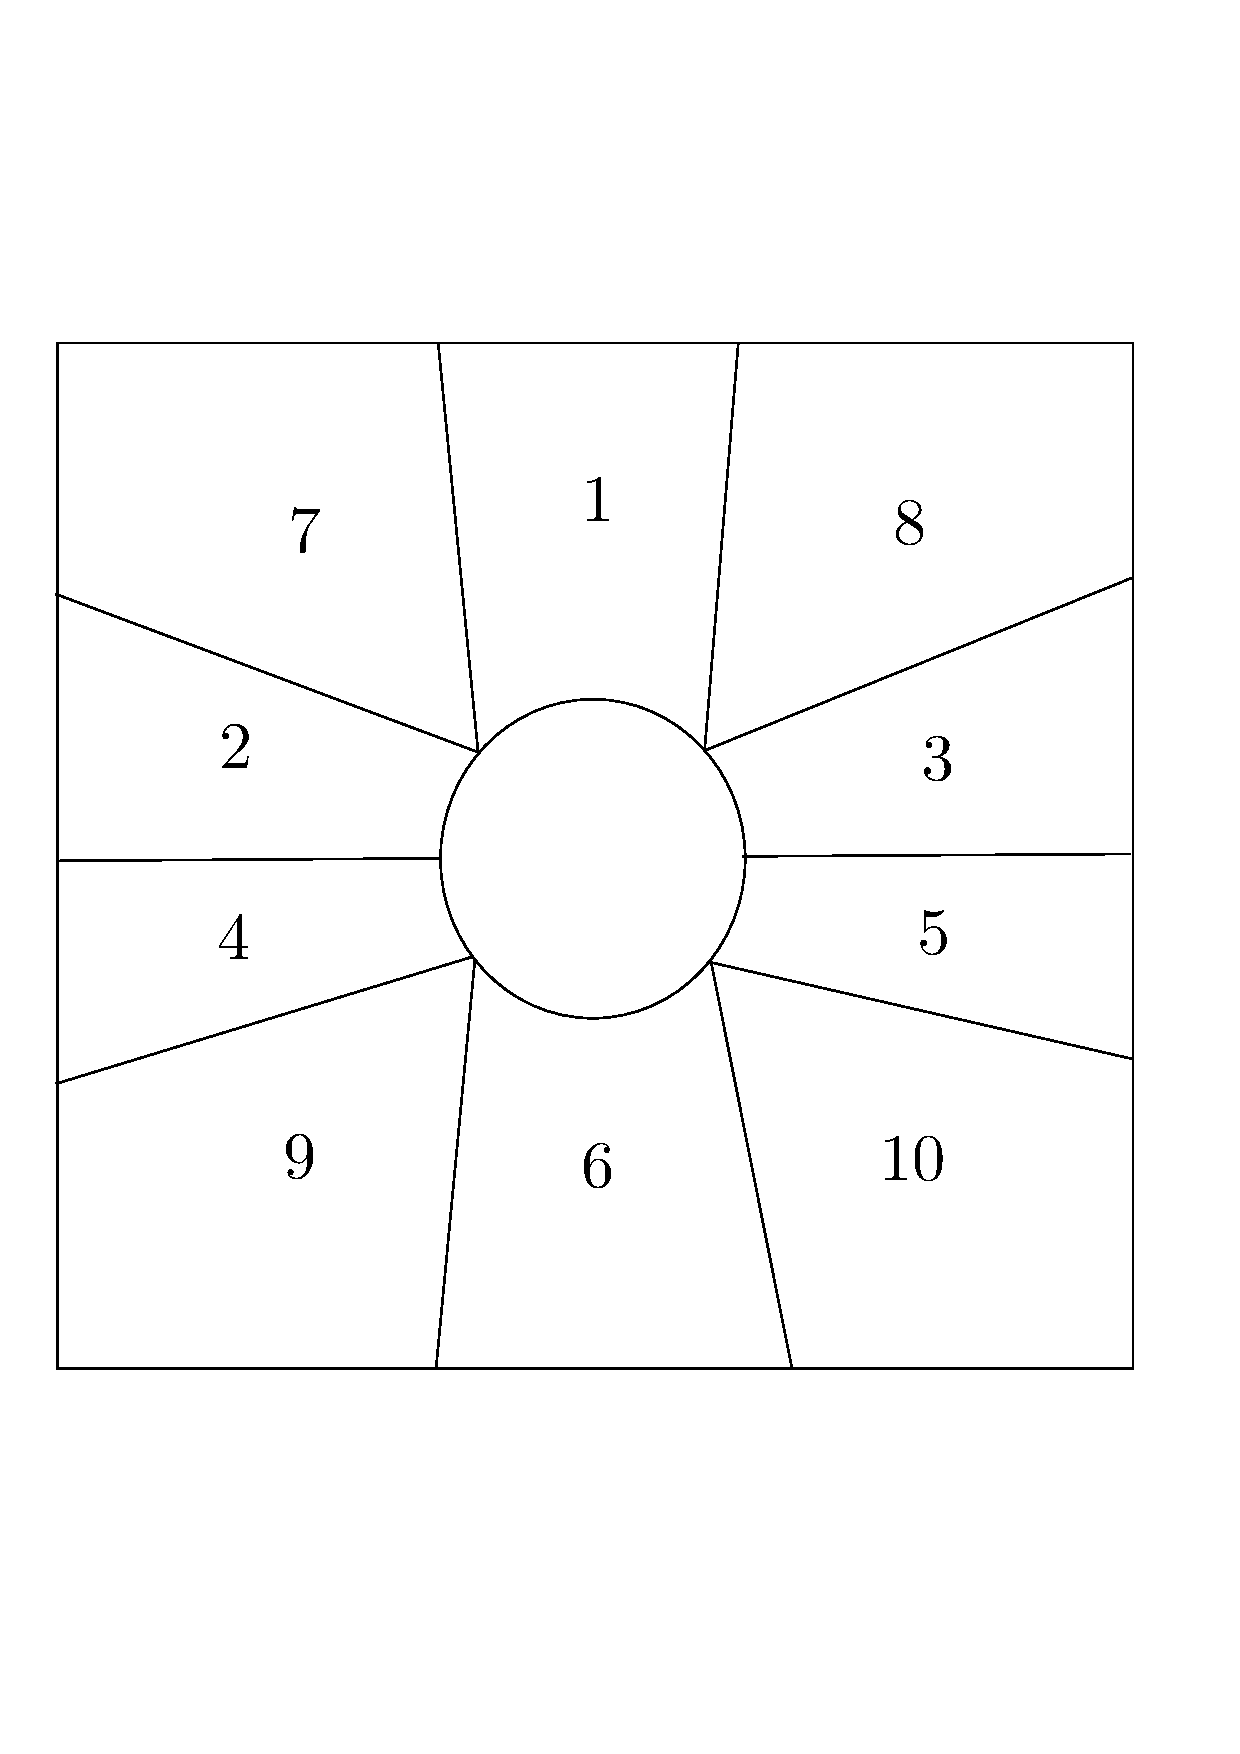
\includegraphics[width = 0.3\textwidth]{Figures/cyl_elem.pdf}
    \caption{Initial mesh around cylinder.}
    \label{fig:cyl_elem}
\end{figure}
%
The mesh around the cylinder is illustrated in figure~\ref{fig:cyl_elem}.
Initially this case was solved using a second degree polynomial to describe the circle segments
corresponding to each element. However with the new routine implemented as described 
in~\ref{xyzarc} the circle segments could be represented with the same order as 
the polynomials used for the velocity space. The importance of the error resulting 
from the second degree approximation of the circle segments are presented in \cref{results}.
%Note that these elements was split in three, in order to obtain 
%a finer mesh in the region of interest. Of the elements numbered in~\ref{fig:cyl_elem}
%only the first six contains edges on the cylinder.Hence the second order polynomials 
%describing the curved edges describe approximately $\Theta = 360^{\circ}/(6\cdot 3) = 20^{\circ}$
%of the complete circle. 

An additional test that is performed on this case is how different settings in Nek5000 will affect the estimation of the drag and lift coefficients.
Perhaps most curious is whether the $P_NP_N$- or $P_NP_{N-2}$ formulation is applied. Note that the pressure in the latter formulation is 
not defined on the boundary of the cylinder and does therefore need to be extrapolated onto the surface in order for the integral to be 
calculated. On the other side is the splitting scheme implied by the $P_NP_N$ known to produce large errors close to the boundary. 

\colorbox{red}{Add some theorem addressing this error difference! }
%

\section{Advances in the mesh-generation routine} \label{xyzarc}

The Gordon Hall (GH) algorithm which is described in~\ref{GH} was already implemented as a function in the Nek library.
By defining the GLL-nodes on the curved edges such that they correspond to an arc, the GH-algorithm is able to distribute 
the internal nodes accordingly. 

The curved edges are specified in \verb|.rea| and have until now been read as a second degree polynomial or as a part of a 
spherical shell. The routine \verb|xyzarc()| was created to process curved edges specified in \verb|.rea| with a radius and center.
The algorithm is described below and figure~\ref{fig:curvature} gives a visual representation of the situation.

$a,b$ will be the two end nodes of the edge, 
$c$ will be the mid node, 
$s$ will be the arc length, 
$\theta$ will be the full angle of the circle sector,
$cc$ is the center coordinates, 
$g$ will be the vector containing the GLL-points in $[-1,1]$ 
and $r$ will be the radius.

\begingroup
%\fontsize{12pt}{14pt}
\begin{lstlisting}[escapechar=|,frame=none]
 l = a-b                       ! vector between the corner nodes
 c = (a+b)/2                   ! midpoint location
 h = c-cc                      ! height of the framed triangle
 |$\theta$| = arctan(abs(l)/2*abs(h))    ! half the angle of the circle sector
 s = r*|$\theta$|                       ! arc length
 g = g*|$\theta$|                      ! angles to the GLL-points on the circle-sector
 !---------- Finding the intersecting points ----------!
 !---- x on the line l, and extend x-cc to the arc ----!
 do k=1,lx1          ! for the number of nodes in one direction
    |$\alpha$| = h*tan(g[k])           ! offset from the midpoint on l
    x = c-|$\alpha$|*l/abs(l)           ! actual coordinate on l
    m = x-cc                   ! hypotenuse of the imposed triangle
    edge(k) = cc+r*m/abs(m)    ! final coordinate on the arc
 enddo
\end{lstlisting}
\endgroup
This code defines the GLL-nodes on a circle sector corresponding to the radius and circle center given.
The remaining operation is to call the Gordon Hall algorithm and create the internal GLL-points.
%
\begin{figure}[h]
    \centering
    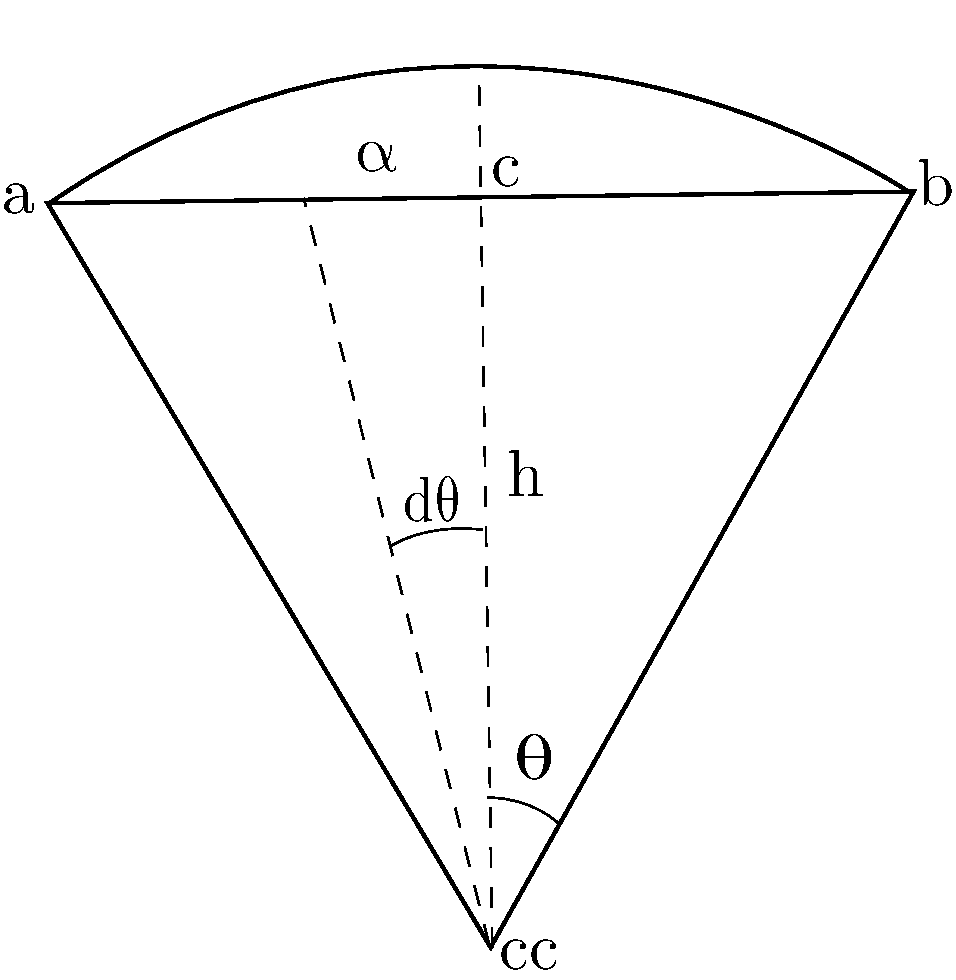
\includegraphics[width = 0.4\textwidth]{Figures/curvature.pdf}
    \caption{A sketch of the curved edge and the variables necessary to calculate the projection}
    \label{fig:curvature}
\end{figure}
%
\section{Additional projection algorithm}\label{surfpro}
The routine \verb|xyzarc()| enables the user to more accurately represent circular edges.
For more complex geometry such as actual terrain and other surfaces without any analytic
expression the large element sizes makes the geometrical representation difficult. 
Theoretically the GLL-points can be projected onto a non-analytical surface, but since 
the element mesh is created in a different program the necessary information is not available
to Nek5000. The idea is to create an additional fine surface mesh in ICEM such
that the nodes in this mesh describes the surface as fine or finer that the final mesh in Nek5000.
During the initialization of the mesh in Nek5000 the program can read this information and project the GLL-nodes onto 
the provided surface. 
The routine was made as automatic as possible, and can be summed up in these four steps
\begin{enumerate}
    \item Create initial Mesh and convert to .rea applying nmshconvert.
        \item Create refined surface mesh on the non-regular surface.
        \item Enable projection by setting param(33) = 1.
        \item Choose number of interpolation points by modifying param(34)= (1,2,3)
\end{enumerate}

In addition to the standard Nek library the file \verb|surfpro.f| needs to be added to 
the folder \verb|/trunk/nek/| along with all the other scripts applied by Nek5000.
This implementation could be done directly in \verb|.usr|, but it is of practical 
interest to keep this file as tidy as possible.
Two external files are also generated by the modified nmshconvert script for the algorithm to work.
\verb|surf.i| contains all the coordinated to the points on the refined surface. 
\verb|bdry.i| contains the element, and face number to all the faces to be projected onto the surface.
%When generated they automatically alter the local \verb|SIZE| file to contain some key variables 
%applied in the algorithm in \verb|surfpro.f|.

The algorithm is best explained through a simple box with a non-regular floor. 
As an initial test-problem the hill of Ekeberg was applied. 
Before describing the algorithm let $E_{tot} = n_xn_yn_z$  be the total number of elements, 
$N$ is the polynomial degree and let us for simplicity assume that $n_x=n_y=n_z$ such that 
$E= E_{tot}^{2/3}$ is the number of elements containing a face on the non-regular surface.
The number of points on the refined surface $N_s$ should be approximately $EN^4$ in 
order to describe the surface for all the GLL-points that belong to the boundary. This estimate
assumes that the surface mesh is equidistantly distributed whereas the GLL-nodes follow a 
quadratic distribution. 

\colorbox{red}{Do I need some reference for this ?}

The pseudo code for the algorithm is listed below with the temporal costs commented out.
%
\begingroup
\fontsize{12pt}{14pt}
\begin{lstlisting}[escapechar=|,frame=none]
do e,f in bdry.i   !O(E)
  wrk = create_working_surface(e,f)  !O(EN^4) 
  do i in GLL-nodes   !O(N^2)
    interp = init_interpolation_array() !O(1) 
    do j in wrk   !O(N^4)
       update_int_array(interp,wrk(j)) ! O(1)
    enddo
    set_new_point(interp,wrk,i,e,f) ! O(1)
  enddo
  fix_GLL() !O(N^3)
enddo
fix_geom()
\end{lstlisting}
\endgroup
% 
In order to understand the algorithm a short description of the auxiliary functions is 
given in the list below
\begin{itemize}
    \item create\_working\_surface(e,f) -- Loops through all the nodes in surf.i and adds the 
        surface-coordinates within a certain radius to the center GLL-node to the array wrk.
        This saves time in the search for interpolation points for each GLL-node.
    \item init\_interpolation\_array() -- initializing the array containing the closest 
        points on the surface for the current GLL-node. 
    \item update\_int\_array(interp,wrk(j)) -- compares the current surface point to the 
        already existing interpolation points and adds it to the list if it is found to 
        be closer to the initial GLL-node.
    \item set\_new\_point(interp,wrk,i,e,f) -- updating the new GLL-point determined by the 
        surface points in interp.
    \item fix\_GLL() -- There is a risk after distributing the GLL-points on the surface that
        some of the internal GLL-points falls outside the element. fix\_GLL() distributes 
        all internal GLL-points correctly between the newly projected face and the opposite.
    \item fix\_geom() -- An already existing Nek routine which redistributes the GLL-points to 
        assure that the distance between them on the new surface are correct.
\end{itemize}

Although this routine is only called once, and therefore will not contribute significantly 
to the total runtime of the program it is desirable to have a fast algorithm. Another analysis
important to be made is the amount of extra storage space needed for this algorithm.
By analysing the pseudo code the time of the algorithm should be of order $O(E(EN^4+N^2N^4+N^3))=O(EN^4(E+N^2))$
and the amount of additional storage space will be of order $O(EN^4+E+N^2)=O(EN^4)$.

The routine attempts to be as automatic as possible and the only implementation necessary is 
a call from \verb|usrdat2| with 3 input variables.

\colorbox{red}{Should this illustrative example be included?}
Now an illustrative example of how this method is applied by the user. Say you have a project
called ''myFlow'', and the mesh and surface mesh created in ICEM are named mesh\_myFlow and 
surfmesh\_myFlow. The following commands are then executed

%
%\begin{lstlisting}[style=FormattedNumber, basicstyle = \ttfamily,frame= none]
%>> ~/path/to/meshconvert/scrpt/nmshconvert --mesh mesh_myFlow 
%--reafile init.rea --outfile myFlow.rea
%--tol 1e3 --temperature True --curvetype A

%>> ~/path/to/meshconvert/scrpt/nmshconvert --mesh surfmesh_myFlow --mesh_format surface
%\end{lstlisting}
% 
\begingroup
\fontsize{12pt}{14pt}
\begin{lstlisting}[escapechar=|,frame=none]
>> /nmshconvert --mesh mesh_myFlow 
    --reafile init.rea --outfile myFlow.rea
    --tol 1e3 --temperature True --curvetype A

>> ./nmshconvert --mesh surfmesh_myFlow 
    --mesh_format surface

\end{lstlisting}
\endgroup
% 
% 
%\begin{lstlisting}[style=FormattedNumber, frame=none]
    %int* p;
    %int a[4];
    %p = a;
%\end{lstlisting}
\subsection{Application on the hill of Ekeberg}
As an initial test of the algorithm a mesh was created based on the hill of Ekeberg.
The surface was loaded as a \verb|.tin| file in ICEM and a simple box was created with 
the described terrain as floor. The domain with the initial mesh in given in 
figure~\ref{fig:ekeberg}. This geometry was chosen because it resembles a typical problem with 
spectral elements. Since the initial element-mesh is relatively coarse it does not capture all 
the details in the geometry and the GLL-nodes distributed on the faces corresponding to the 
unstructured surface will be misplaced. 
%It is however no theoretical problem to reconstruct the surface with with a polynomial of order $P$. 
With the routine described in \cref{surfpro} the surface was approximated accurately by higher order polynomials.
%
\begin{figure}[t]
    \centering
	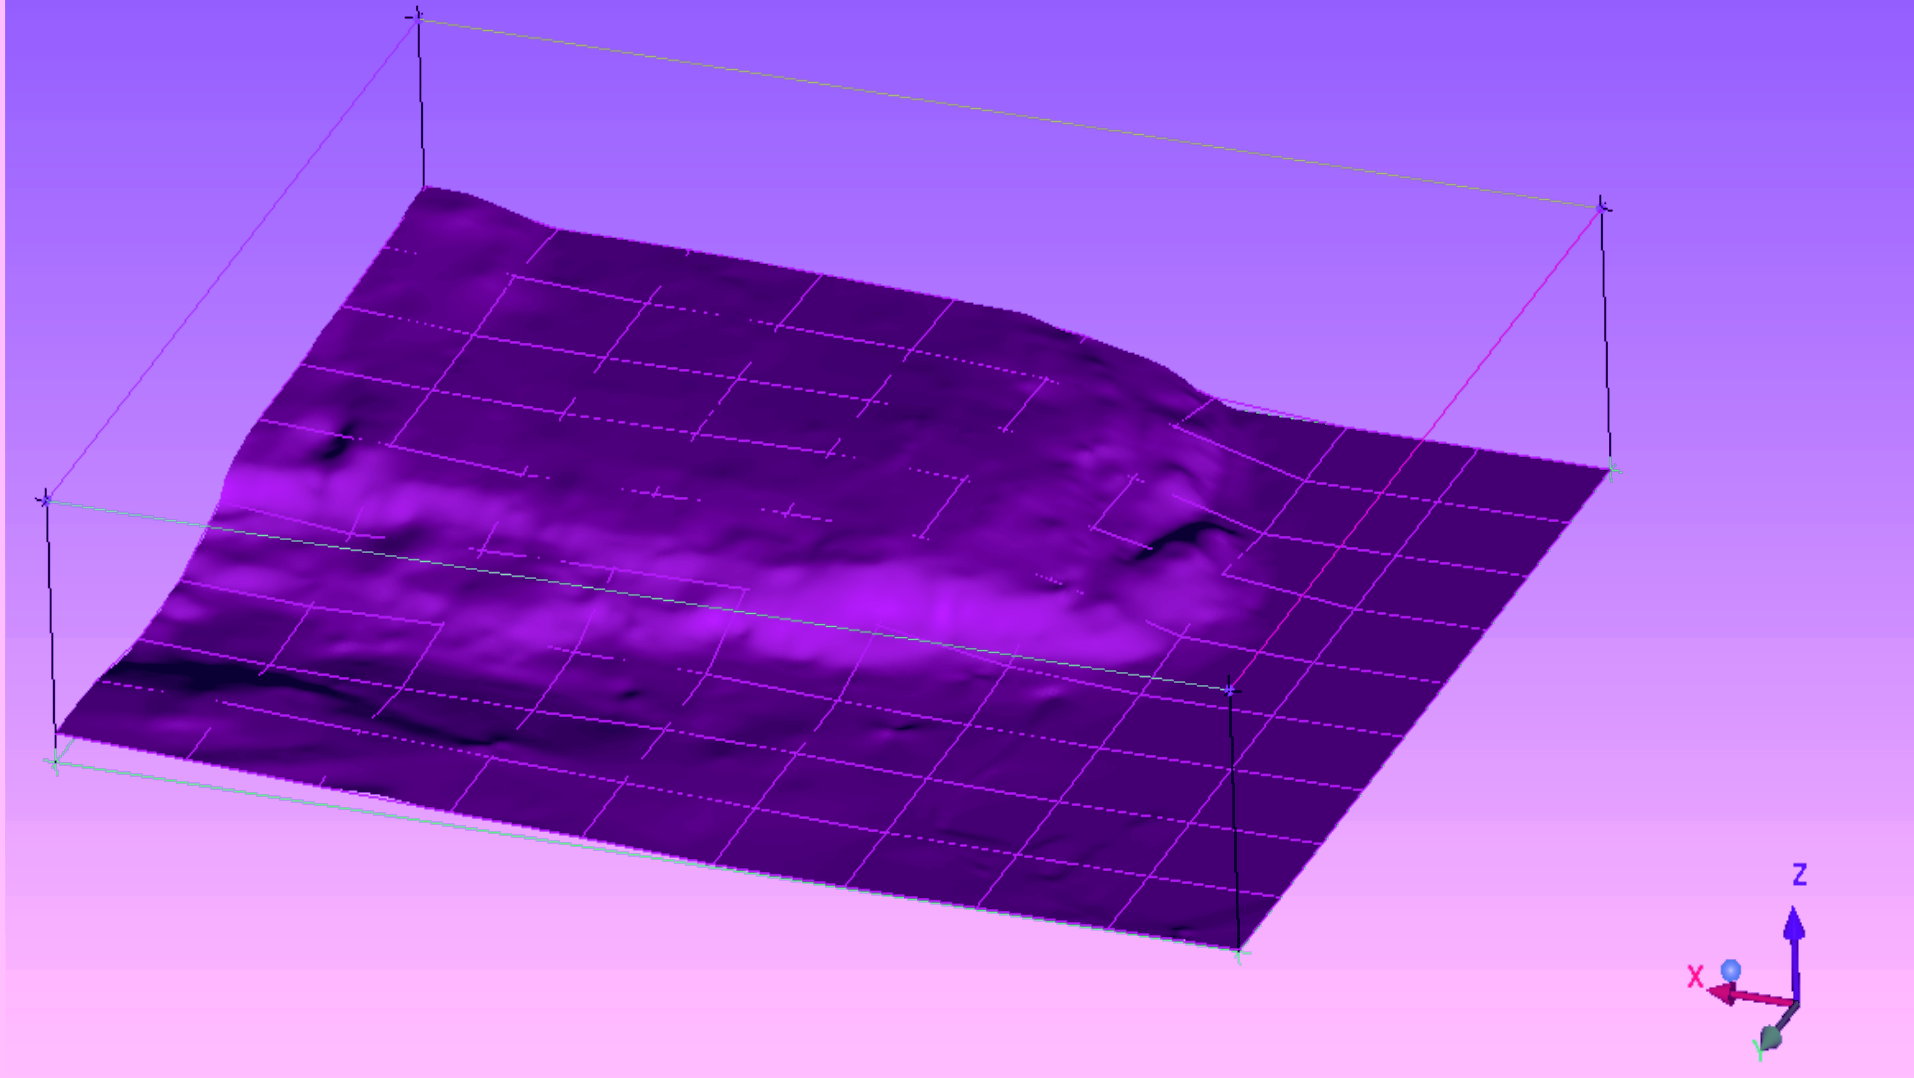
\includegraphics[width=0.7\textwidth]{Figures/mesh_ekebergaasen2.png}
    \caption{The initial mesh of the hill}
	\label{fig:ekeberg}
\end{figure}
%
%
\begin{figure}[t]
    \centering
	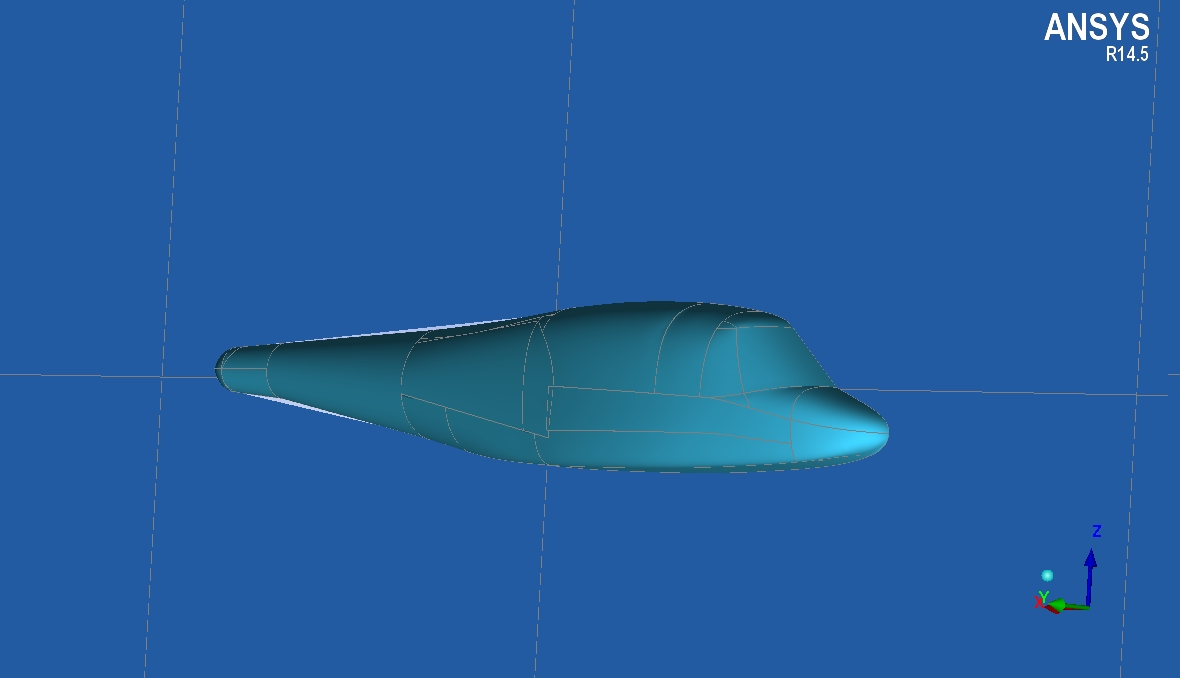
\includegraphics[width=0.7\textwidth]{Figures/helicopter.jpg}
    \caption{Body of a helicopter}
	\label{fig:helicopter}
\end{figure}
%
%
\begin{figure}
\centering
  \centerline{
\begin{minipage}{.6\textwidth}
  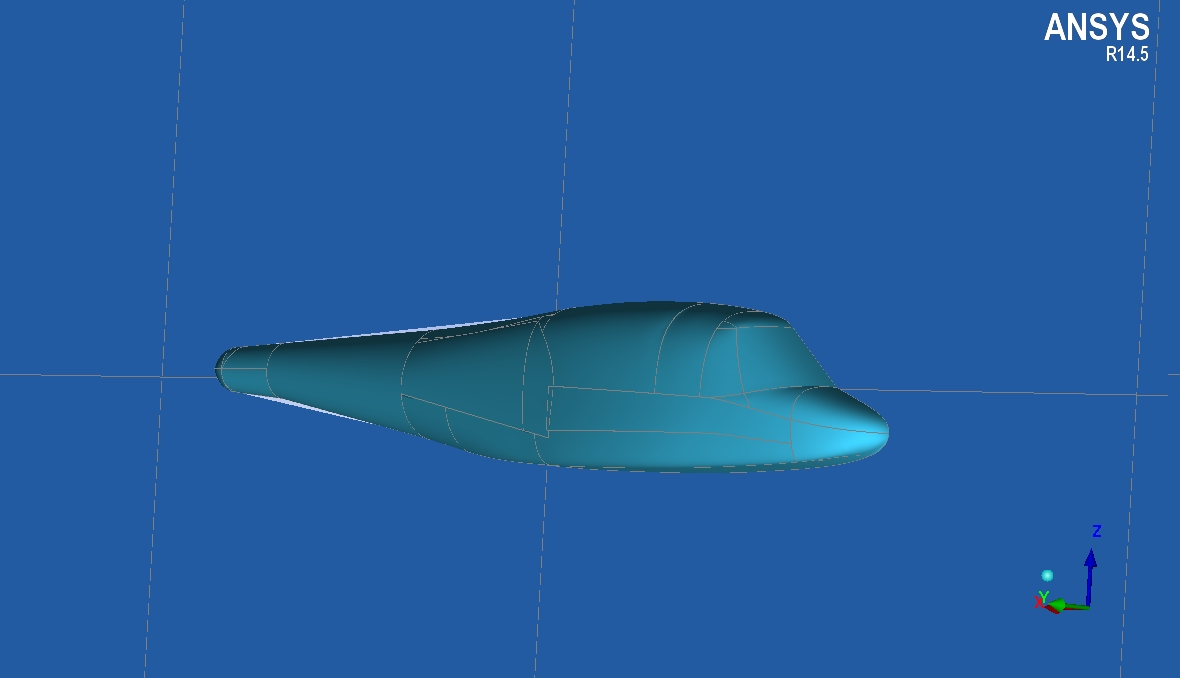
\includegraphics[width=1.0\linewidth]{Figures/helicopter.jpg}
  %\captionof{figure}{A figure}
\end{minipage}%
\begin{minipage}{.6\textwidth}
  \centering
  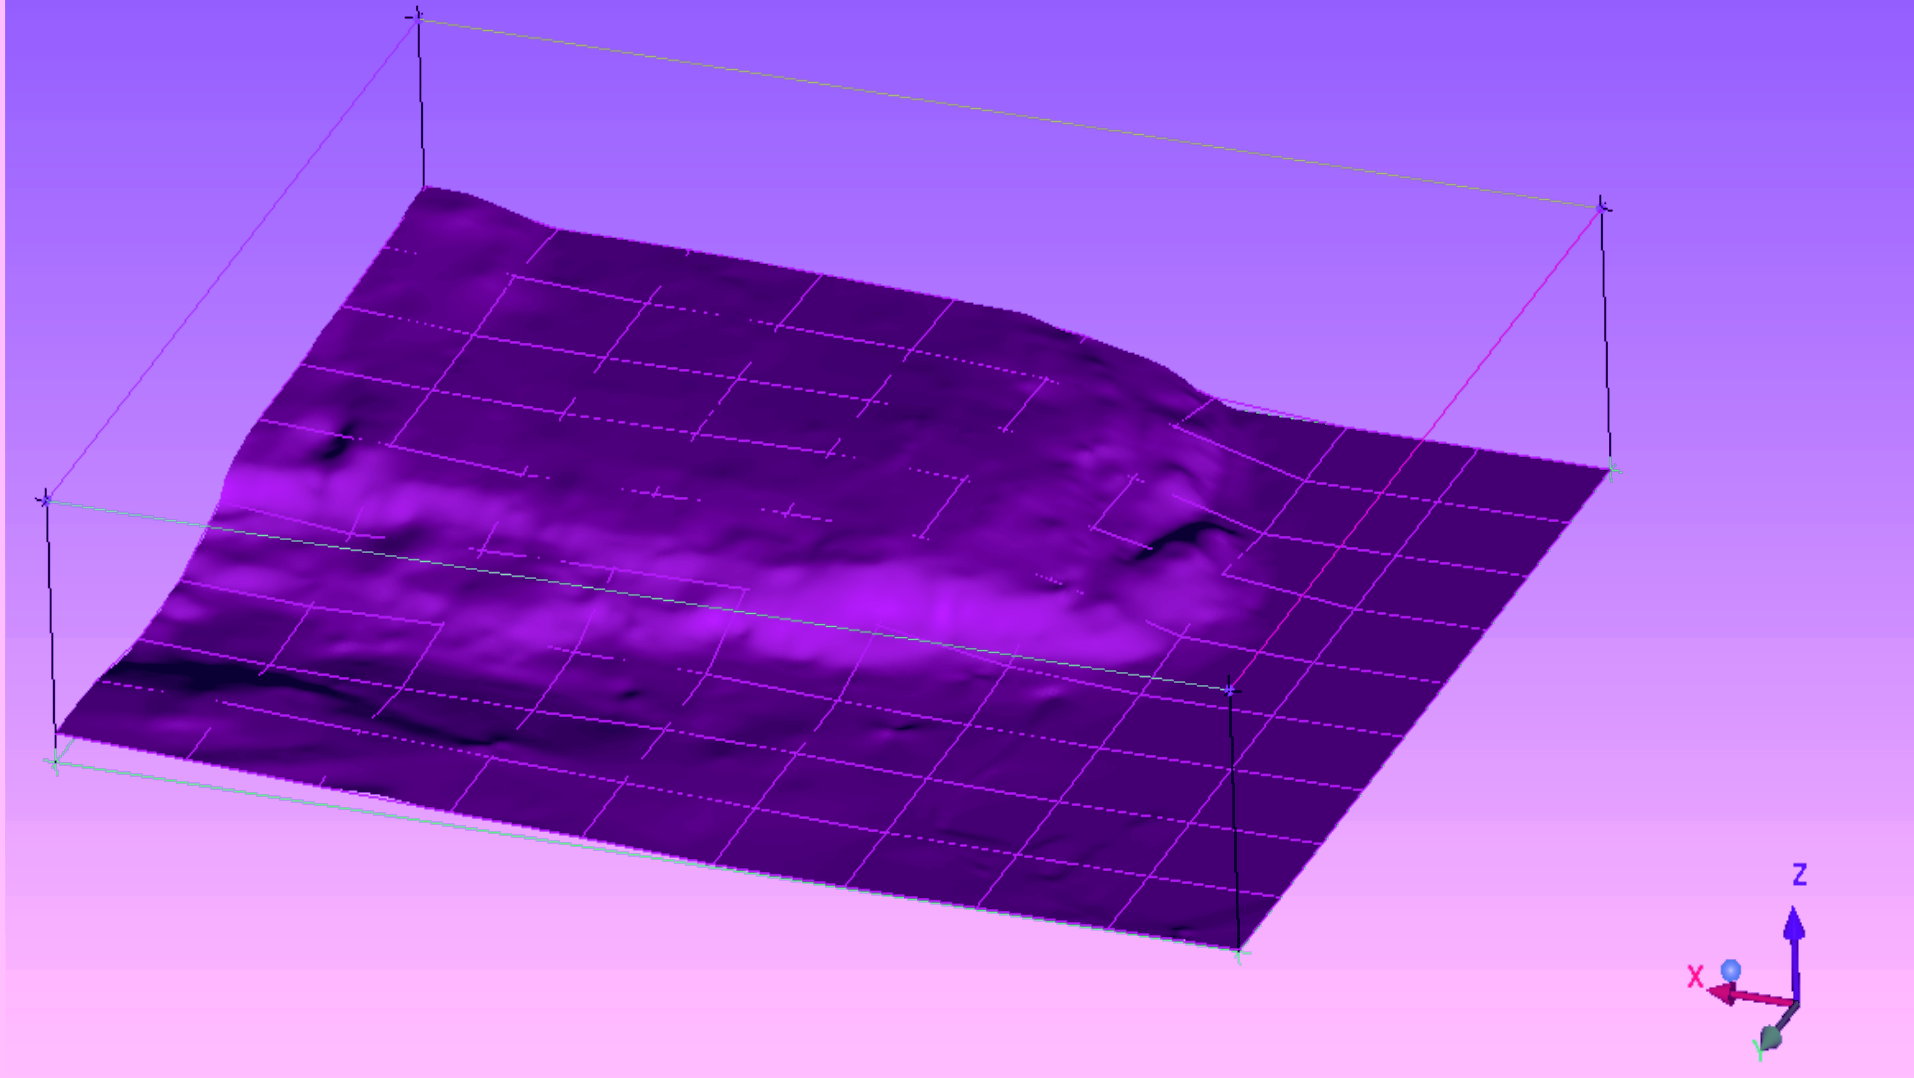
\includegraphics[width=1.0\linewidth]{Figures/mesh_ekebergaasen2.png}
\end{minipage}
}
  \caption{The averaged (left) and instantaneous (right) x-velocity on the inflow boundary.}
  \label{fig:surfpro}
\end{figure}
%
The algorithm restricts itself to relatively smooth surfaces.
\colorbox{red}{add this section to the results part with other applications as well??}
\section{Spatial averaging routine}
A dynamic Smagorinsky model has previously been implemented in Nek5000 for flow in a channel. 
The SGS-model as described in \cref{description} depends on an averaging routine to calculate
the dynamic Smagorinsky constant. The previous implementation in Nek applies an average routine in the plane,
assuming that the Smagorinsky constant is the same for all points with equal distance to the walls 
of the channel. This is a rather specific averaging routine based on the assumption of homogenous turbulence 
in the entire plane, hence only applicable to flows in idealized geometries.

When applying dynamical Smagorinsky to Case 1 a new spatial mean routine had to be applied for it to be stable. 
It was first attempted to average only in time, but this proved not to be sufficient. It was
therefore implemented a routine for taking the average within each element, let 
$c_{num}^e,c_{den}^e$ denote the numerator and the denominator in \eref{eq:dynsmag}.
The means are then calculated as 
\begin{align}
    c_{num}^e = \frac{1}{V}\int_{\Omega_e}c_{num}^e d\: \Omega 
    = \frac{1}{V}\sum_{i = 1}^{N^3}\rho_{i,e}c_{num,i}^{e}.
    \label{eq:averageroutine}
\end{align}
And similarly for $c_{den}^e$.
The coefficients $\rho_{i,e}$ are found in the array \verb|BM1(lx1,ly1,lz1)| in the file 
\verb|MASS|.
